\subsection{The Cable Theory}
\subsubsection{Introduction}
The Cable Theory, first developed in 1850s and applied to neuroscience in 1930s and 1940s,
is based on a strong assumption: neuronal processes contain only voltage-independent
components. In other words, neurons are assumed to work exclusively as passive components,
therefore only resistances and capacitances are considered.\\
The following quantities represents the electrical components involved in the Cable Theory.
\begin{figure}[H]
    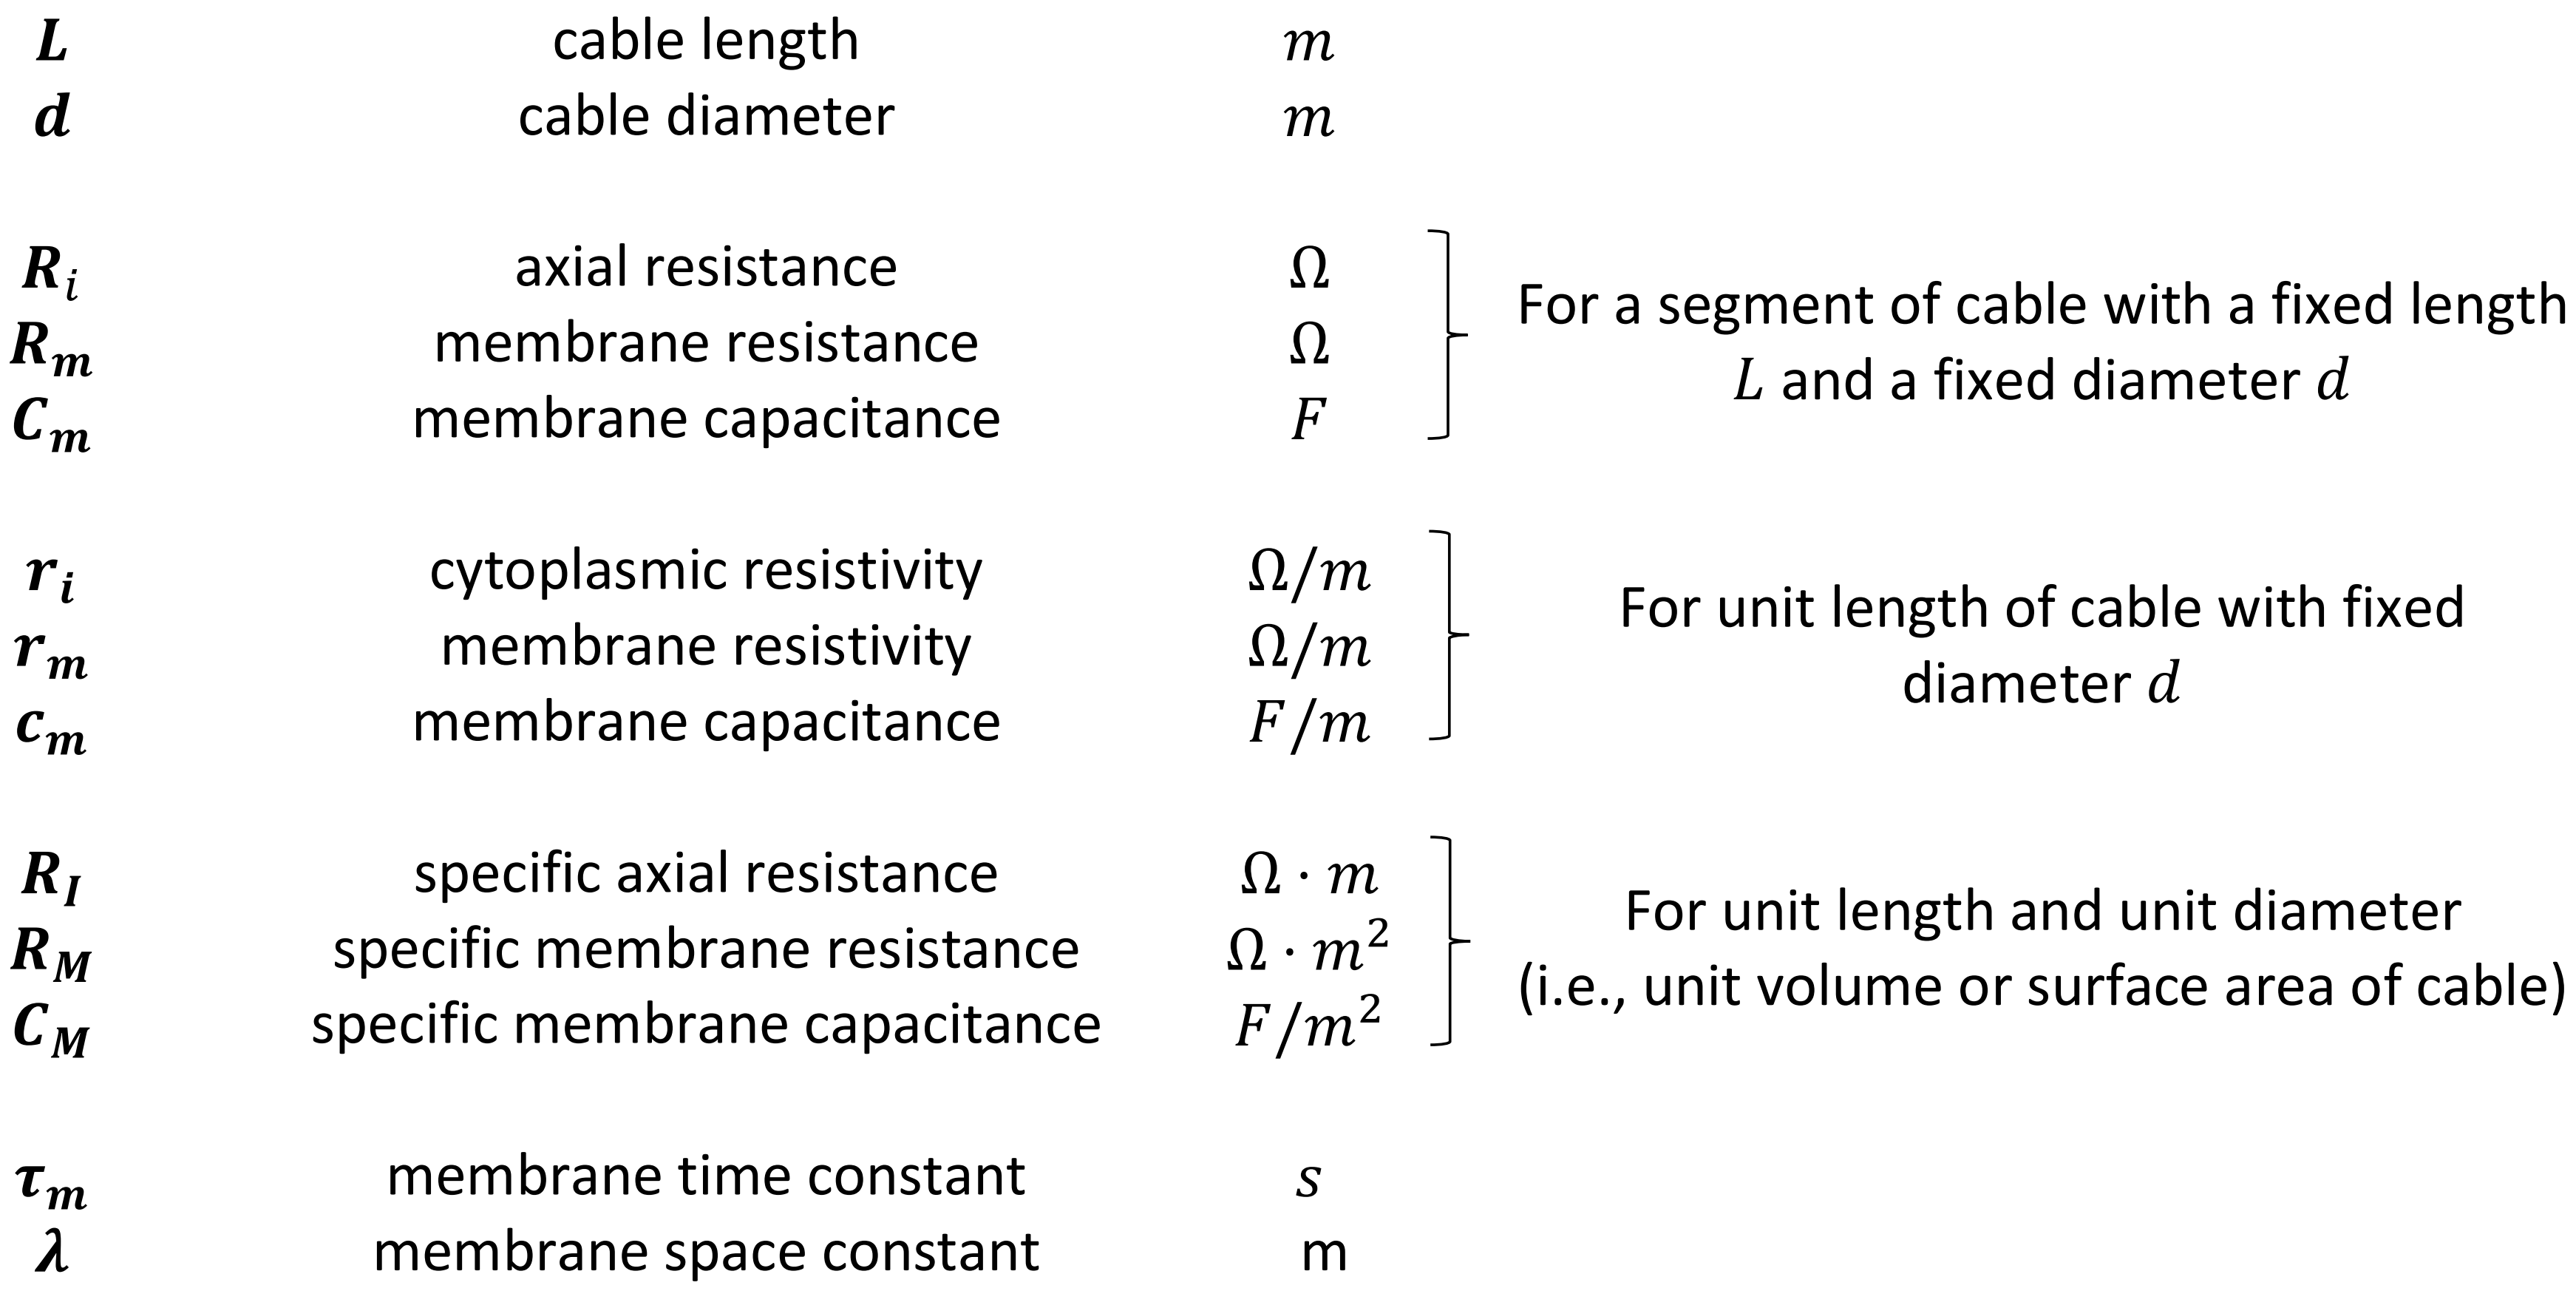
\includegraphics[scale=0.18]{04_1}
    \centering
\end{figure}
Note that given these measures, the relatonships reported here hold:
\begin{gather*}
    R_{i}=r_{i}L=\frac{4L}{\pi{d^2}}R_{I}
    \hspace{2cm}
    R_{m}=\frac{r_{m}}{L}=\frac{R_{M}}{\pi{dL}}
    \hspace{2cm}
    C_{m}=c_{m}L=\pi{dLC_{M}}\\
    \lambda=\sqrt{\frac{r_{m}}{r_{i}}}=\sqrt{\frac{d}{4}\frac{R_{M}}{R_{I}}}
    \hspace{2.5cm}
    \tau_{m}=r_{m}c_{m}=R_{M}C_{M}=R_{m}C_{m}
\end{gather*}
The cable is modelled as depicted below and the subsequent canonical expression for
the cable equation is derived.
\begin{figure}[H]
    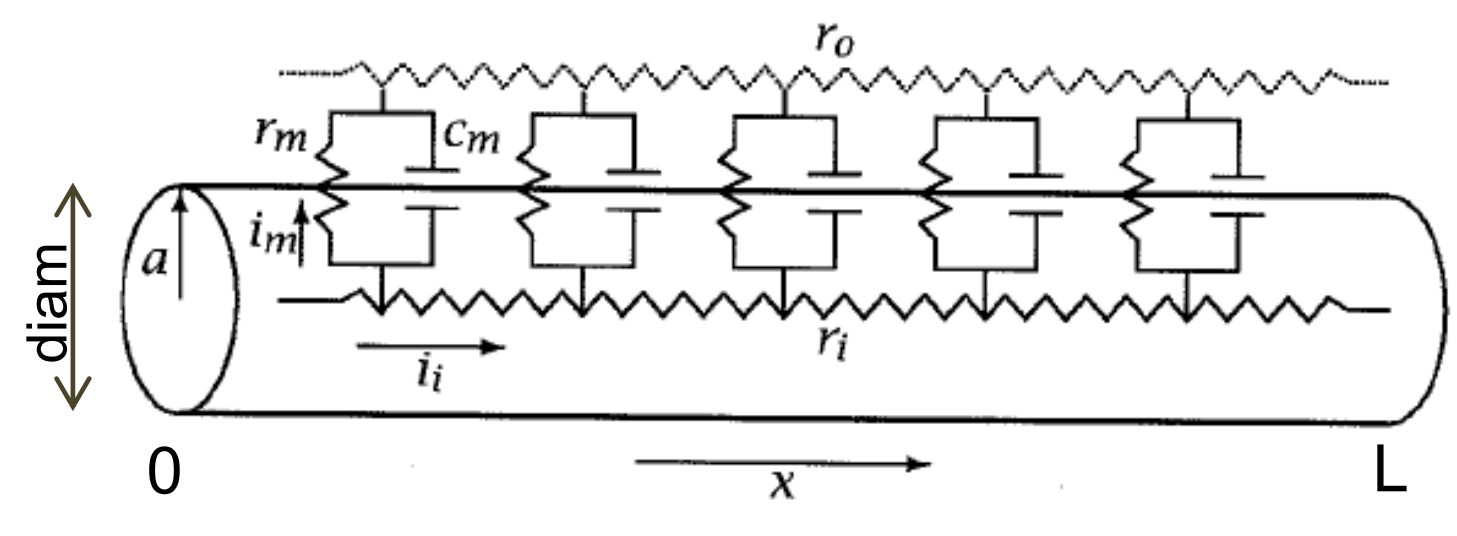
\includegraphics[scale=0.26]{04_2}
    \centering
\end{figure}
\begin{equation*}
    \lambda^{2}\frac{\partial^{2}V}{\partial{x^{2}}}-V-\tau{\frac{\partial{V}}{\partial{t}}}=0
    \Rightarrow
    \frac{\partial^{2}V}{\partial{X^{2}}}-V-\frac{\partial{V}}{\partial{T}}=0
\end{equation*}
Note that \(X=\frac{x}{\lambda}\) and \(T=\frac{t}{\tau}\), while \(V=(V_{i}-V_{e})-E_{r}\), with
\(V_i\) being the intracellular potential and \(V_e\) the extracellular one.
\subsubsection{Proof (Cable Equation Derivation)}
First of all, it is important to establish some hypotheses:
\begin{itemize}
    \item Neuronal processes contain only voltage-independent components, thus only passive
          electrical quantities are considered.
    \item The neurite is short (either axon or dendrites): \(L<\lambda\).
    \item The neurite length is much greater than its diameter: \(L>>d\).
    \item The propagation of the current is longitudinal, thus the current flows in parallel
          to the cylinder axis: \(r_{m}>>r_{i}\).
    \item The electrical properties of the membranes (\(r_{m}\), \(r_{i}\), \(c_{m}\)) are
          assumed to be uniform: \(V=V(t,x)\).
\end{itemize}
\begin{figure}[H]
    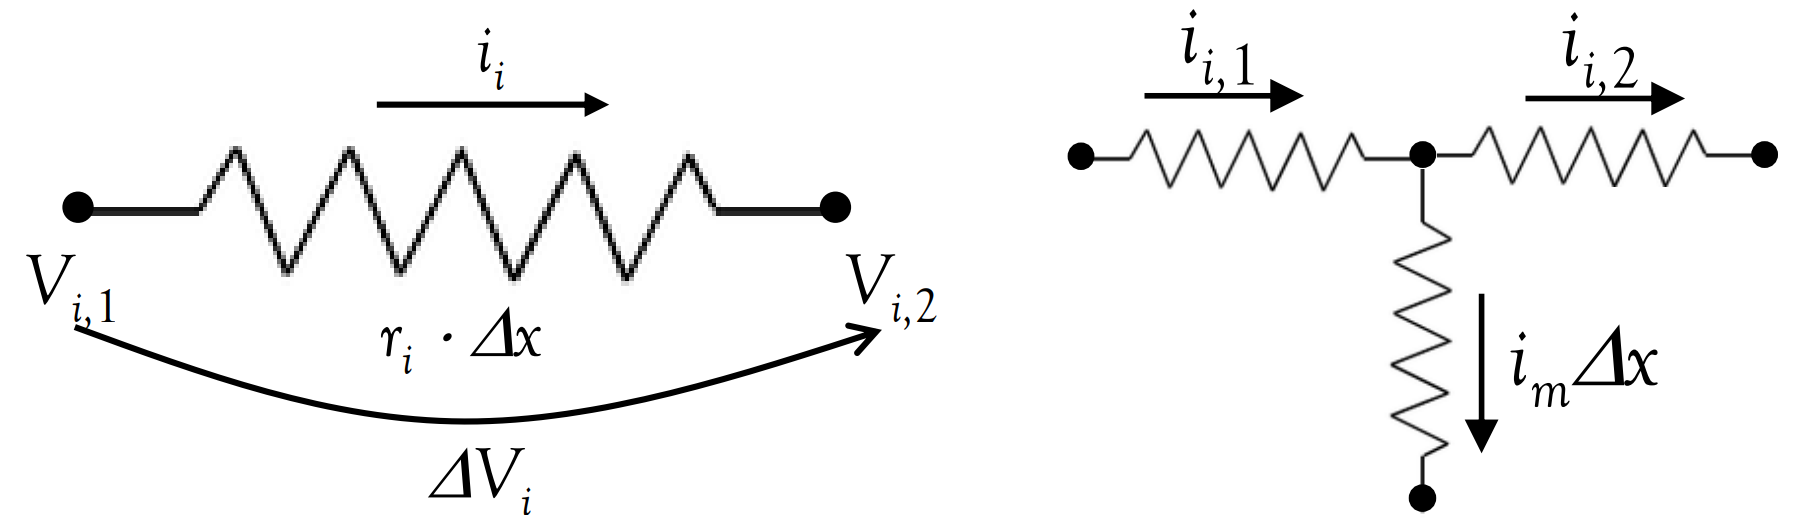
\includegraphics[scale=0.3]{04_3}
    \centering
\end{figure}
Due to the Ohm's Law:
\begin{equation*}
    i_{i}(r_{i}\Delta{x})=-\Delta{V_{i}}\Rightarrow\frac{\Delta{V_{i}}}{\Delta{x}}=-r_{i}i_{i}
\end{equation*}
Note that if \(\Delta{x}\) is infinitesimal (\(\Delta{x}\to{0}\)), this expression changes as:
\begin{equation*}
    \frac{\Delta{V_{i}}}{\Delta{x}}=-r_{i}i_{i}\Rightarrow\frac{\partial{V_{i}}}{\partial{x}}=-r_{i}i_{i}
\end{equation*}
Let's now derive the whole expression once again, without forgetting that \(r_{i}\) is uniform
by hypothesis:
\begin{equation*}
    \frac{\partial{V_{i}}}{\partial{x}}=-r_{i}i_{i}
    \Rightarrow
    \frac{\partial^{2}V_{i}}{\partial{x^{2}}}=-\frac{\partial{r_{i}i_{i}}}{\partial{x}}
    \Rightarrow
    \frac{\partial^{2}V_{i}}{\partial{x^{2}}}=-r_{i}\frac{\partial{i_{i}}}{\partial{x}}
\end{equation*}
At this point, some considerations can be done:
\begin{itemize}
    \item \(\frac{\partial{i_{i}}}{\partial{x}}=0\): there are no current variations
          within the increment \(\Delta{x}\).
    \item \(\frac{\partial{i_{i}}}{\partial{x}}<0\Rightarrow\frac{\partial^{2}V_{i}}{\partial{x^{2}}}>0\):
          there is an excess of current in the increment \(\Delta{x}\), thus an outward current \(i_{m}\) should
          be accounted for.
    \item \(\frac{\partial{i_{i}}}{\partial{x}}>0\Rightarrow\frac{\partial^{2}V_{i}}{\partial{x^{2}}}<0\):
          there is an entering current in the increment \(\Delta{x}\), indicating the presence of a synapse.
\end{itemize}
By applying the KCL, one can write that
\begin{equation*}
    i_{i,2}-i_{i,1}=-i_{m}\Delta{x}
    \Rightarrow
    \Delta{i_{i}}=-i_{m}\Delta{x}
    \Rightarrow
    -\frac{\Delta{i_{i}}}{\Delta{x}}=i_{m}
\end{equation*}
and if \(\Delta{x}\to{0}\) it becomes the following:
\begin{equation*}
    -\frac{\Delta{i_{i}}}{\Delta{x}}=i_{m}
    \Rightarrow
    -\frac{\partial{i_{i}}}{\partial{x}}=i_{m}
\end{equation*}
At this point, the resulting expression can be substituted into the previous one, leading to:
\begin{equation*}
    \frac{\partial^{2}V_{i}}{\partial{x^{2}}}=-r_{i}\frac{\partial{i_{i}}}{\partial{x}}
    \Rightarrow
    \frac{\partial^{2}V_{i}}{\partial{x^{2}}}=r_{i}i_{m}
    \Rightarrow
    \frac{1}{r_{i}}\frac{\partial^{2}V_{i}}{\partial{x^{2}}}=i_{m}
\end{equation*}
By reconsidering once again the previous hypotheses, it has been said that \(V=(V_{i}-V_{e})-E_{r}=V(x,t)\),
however the extracellular liquid is assumed to be isopotential, thus \(V_{e}\) and \(E_{r}\) are
independent on space \(x\) and time \(t\). As a consequence:
\begin{equation*}
    V=(V_{i}-V_{e})-E_{r}
    \Rightarrow
    V_{i}=V+V_{e}+E_{r}
    \Rightarrow
    \frac{\partial{V_{i}}}{\partial{x}}=\frac{\partial{V}}{\partial{x}}
\end{equation*}
Let's now take the previous equation and multiply it by \(r_{m}\):
\begin{equation*}
    \frac{1}{r_{i}}\frac{\partial^{2}V_{i}}{\partial{x^{2}}}\cdot{r_{m}}=i_{m}\cdot{r_{m}}
    \Rightarrow
    \frac{r_{m}}{r_{i}}\frac{\partial^{2}V}{\partial{x^{2}}}=r_{m}i_{m}
\end{equation*}
From now on, the \(i\)-th compartment depicted below is considered.
\begin{figure}[H]
    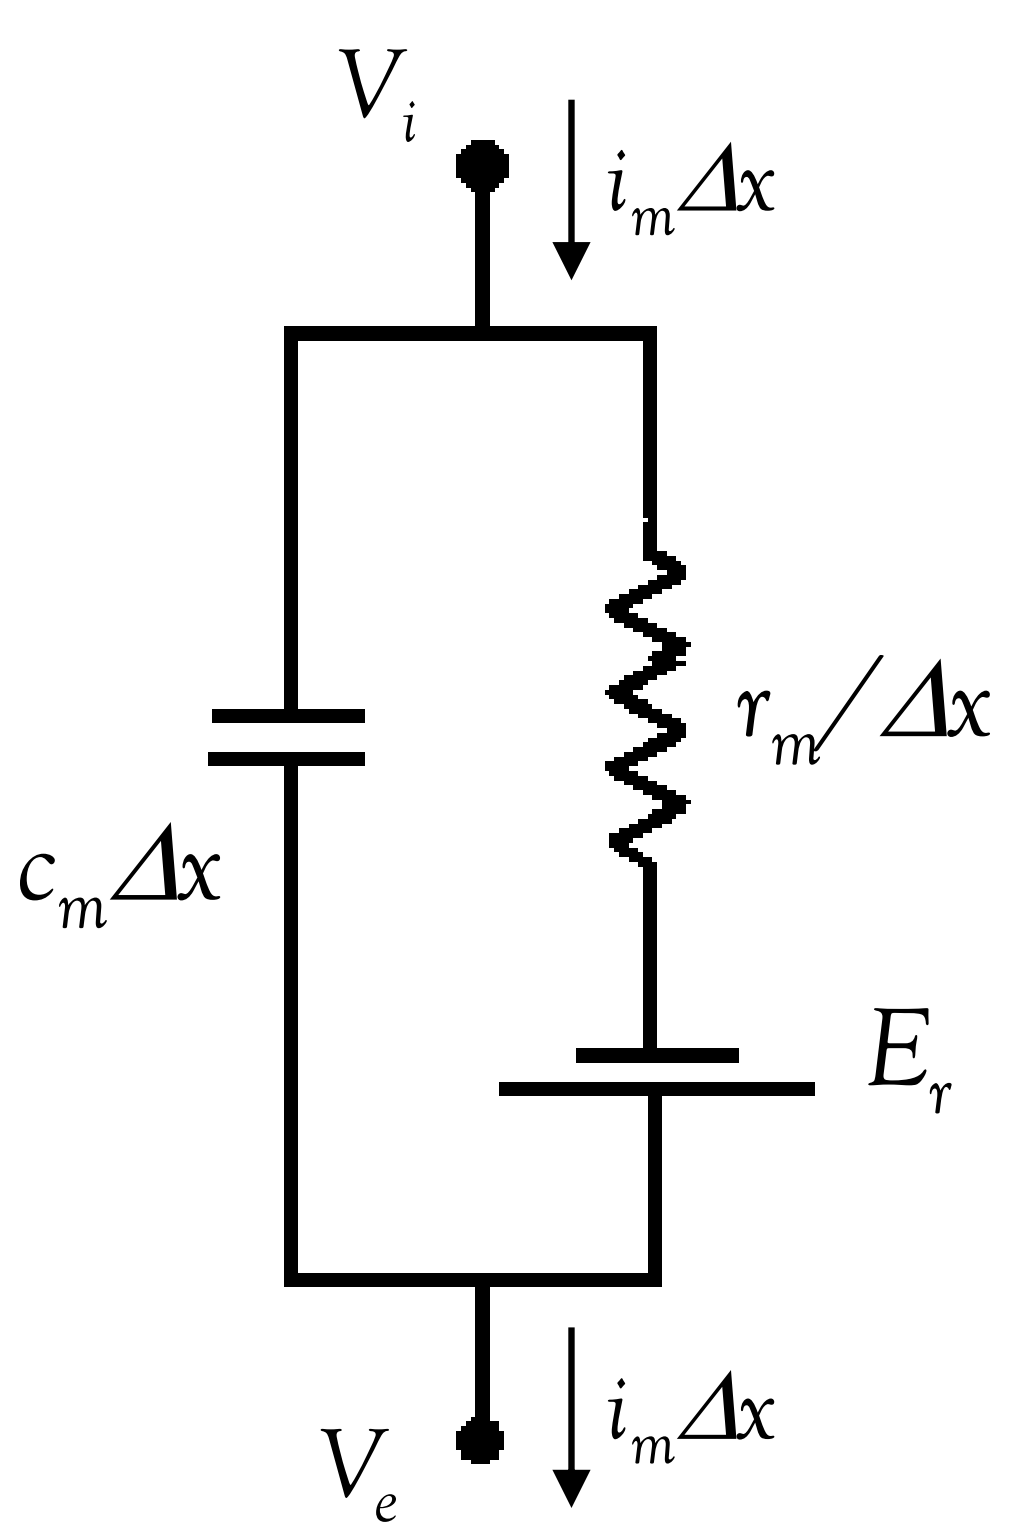
\includegraphics[scale=0.22]{04_4}
    \centering
\end{figure}
By considering its state equation, it can be said that:
\begin{equation*}
    i_{m}=c_{m}\frac{\partial{V}}{\partial{t}}+\frac{(V_{i}-V_{e})-E_{r}}{r_{m}}
    \Rightarrow
    r_{m}i_{m}=r_{m}c_{m}\frac{\partial{V}}{\partial{t}}+V
    \Rightarrow
    r_{m}i_{m}=\tau_{m}\frac{\partial{V}}{\partial{t}}+V
\end{equation*}
as the time constant is defined as \(\tau_{m}=r_{m}c_{m}\).\\
Since
\begin{equation*}
    \frac{r_{m}}{r_{i}}\frac{\partial^{2}V}{\partial{x^{2}}}=r_{m}i_{m}
    \hspace{1.5cm}
    \text{and}
    \hspace{1.5cm}
    \tau_{m}\frac{\partial{V}}{\partial{t}}+V=r_{m}i_{m}
\end{equation*}
it can be easily derived that
\begin{equation*}
    \frac{r_{m}}{r_{i}}\frac{\partial^{2}V}{\partial{x^{2}}}
    =
    \tau_{m}\frac{\partial{V}}{\partial{t}}+V
    \Rightarrow
    \lambda^{2}\frac{\partial^{2}V}{\partial{x^{2}}}-V-\tau_{m}\frac{\partial{V}}{\partial{t}}
    =
    0
\end{equation*}
with \(\lambda=\sqrt{\frac{r_{m}}{r_{i}}}\) being the space constant.
\subsubsection{Space and Time Constants}
\begin{itemize}
    \item \textbf{Space constant \(\lambda\)}: it depends not only on the axoplasmatic
          and membrane resistances (\(r_{i}\) and \(r_{m}\) respectively), but on the cable
          diameter as well, as illustrated by this relationship:
          \begin{equation*}
              \lambda=\sqrt{\frac{r_{m}}{r_{i}}}=\sqrt{\frac{R_{m}}{R_{i}}\frac{d}{4}}
          \end{equation*}
          In particular, cylinders with a bigger diameter tends to exhibit a bigger
          spatial constant, implying that the signal needs a greater distance to be attenuated.
    \item \textbf{Time constant \(\tau\)}: it defines the transient voltage response
          of a segment of the membrane to a current step input. It is formalized as:
          \begin{equation*}
              \tau=\tau_{m}=r_{m}c_{m}=R_{m}C_{m}=R_{M}C_{M}
          \end{equation*}
          Note that a bigger - i.e., slower - time constant implies a slower response to a
          changing stimulus.
\end{itemize}
Note that the \(\frac{\tau}{\lambda}\) ratio represents the time required for the voltage
across the membrane to reach \(\frac{1}{e}=0.37\) of its final value.\\
The obtained equivalent expressions
\begin{equation*}
    \lambda^{2}\frac{\partial^{2}{V}}{\partial{x^{2}}}-V-\tau\frac{\partial{V}}{\partial{t}}=0
    \hspace{2cm}
    \text{and}
    \hspace{2cm}
    \frac{\partial^{2}{V}}{\partial{X^{2}}}-V-\frac{\partial{V}}{\partial{T}}=0
\end{equation*}
are Partial Differential Equations (PDEs) and they were derived under the crucial
assumption that the axoplasmatic resistance \(r_{i}\) is uniform and constant: without this
hypothesis it is much more difficult to find a solution for the differential equation, as the
following term would change.
\begin{equation*}
    \frac{\partial^{2}V_{i}}{\partial{x^{2}}}=-r_{i}\frac{\partial{i_{i}}}{\partial{x}}
    \Rightarrow
    \frac{\partial^{2}V_{i}}{\partial{x^{2}}}=
    -r_{i}\frac{\partial{i_{i}}}{\partial{x}}-i_{i}\frac{\partial{r_{i}}}{\partial{x}}
\end{equation*}
As differential equations and time are involved, two kinds of solutions should be taken into
account:
\begin{itemize}
    \item \textbf{Steady-state solutions}
    \item \textbf{Time-dependent solutions}
\end{itemize}
\subsubsection{Cable Equation Steady-State Solutions}
In steady-state conditions, there is no change of voltage over time, therefore
the cable equation becomes an Ordinary Differential Equation (ODE):
\begin{equation*}
    \frac{\partial^{2}{V}}{\partial{X^{2}}}-V-\cancel{\frac{\partial{V}}{\partial{T}}}=0
    \Rightarrow
    \frac{\partial^{2}{V}}{\partial{X^{2}}}-V=0
\end{equation*}
The solution of such ODE can be equivalently expressed as:
\begin{itemize}
    \item \(V(X)=A_{1}e^{X}+A_{2}e^{-X}\)
    \item \(V(X)=B_{1}\cosh{(X)}+B_{2}\sinh{(X)}\)
    \item \(V(X)=C_{1}\cosh{(L-X)}+C_{2}\sinh{(L-X)}\)
\end{itemize}
where \(X=\frac{x}{\lambda}\) is the electrotonic coordinate and \(L=\frac{l}{\lambda}\)
is the electrotonic distance. Note that the solution will exhibit a sort of
expotential decay as the distance \(x\) from the input point increases.
\begin{figure}[H]
    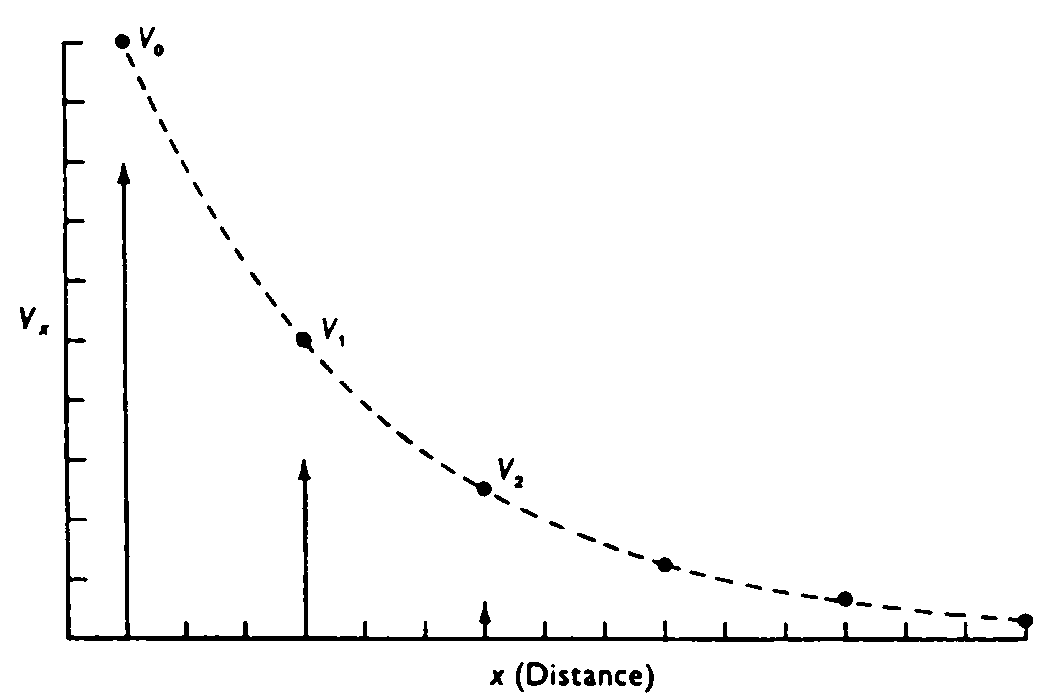
\includegraphics[scale=0.4]{04_5}
    \centering
\end{figure}
Several cases are considered in the following.
\paragraph{Semi-Infinite Cable} This model is not closed on the end side. The voltage
decays exponentially to zero as the distance from the current injection site is increased,
with a rate controlled by the space constant \(\lambda\).\\
\textit{Boundary Conditions:}
\begin{itemize}
    \item \(V(0)=V_{0}=\text{initial voltage}\)
    \item \(V(\infty)=0\)
\end{itemize}
\textit{General Solution:} \(V(X)=A_{1}e^{X}+A_{2}e^{-X}\)\\
\textit{Computations:}
\begin{gather*}
    V(X)\xrightarrow{X\to{\infty}}{0}
    \Rightarrow{0=A_{1}e^{X}+\cancelto{0}{A_{2}e^{-X}}}
    \Rightarrow{A_{1}e^{\infty}=0}
    \Rightarrow{A_{1}=0}\\
    V(X)\mid{}_{X=0}=V_{0}
    \Rightarrow{V_{0}=\cancel{A_{1}}+A_{2}}
    \Rightarrow{A_{2}=V_{0}}
\end{gather*}
\textit{Steady-State Solution:}
\begin{equation*}
    V(X)=V_{0}e^{-X}=V_{0}e^{-\frac{x}{\lambda}}
\end{equation*}
\paragraph{Finite Cable with Sealed End} The end of the cable is closed by an infinte
resistance \(R_{m}\), thus no axial current \(i_{i}\) flows at the end.\\
\textit{Boundary Conditions:}
\begin{itemize}
    \item \(V(0)=V_{0}=\text{initial voltage}\)
    \item \(i_{i}(L)=0\Rightarrow{\frac{\partial{V}}{\partial{X}}\mid{}_{X=L}=0}\)
\end{itemize}
\textit{General Solution:} \(V(X)=C_{1}\cosh{(L-X)}+C_{2}\sinh{(L-X)}\)\\
\textit{Computations:}
\begin{gather*}
    \frac{\partial{V}}{\partial{X}}\mid{}_{X=L}=0
    \Rightarrow{0=-\cancel{C_{1}\sinh{(L-L)}}-C_{2}\cosh{(L-L)}}
    \Rightarrow{0=C_{2}\cancelto{1}{\cosh{(0)}}}
    \Rightarrow{C_{2}=0}\\
    V(0)=V_{0}
    \Rightarrow{C_{1}\cosh{(L)}+\cancel{C_{2}\sinh{(L)}}}
    \Rightarrow{C_{1}=\frac{V_{0}}{\cosh{(L)}}}
\end{gather*}
\textit{Steady-State Solution:}
\begin{equation*}
    V(X)=V_{0}\frac{\cosh{(L-X)}}{\cosh{(L)}}
\end{equation*}
\paragraph{Finite Cable with Open End} This model is cut open at the end, providing
a short circuit to the ground - i.e., the extracellular potential.\\
\textit{Boundary Conditions:}
\begin{itemize}
    \item \(V(0)=V_{0}=\text{initial voltage}\)
    \item \(V(L)=0\)
\end{itemize}
\textit{General Solution:} \(V(X)=C_{1}\cosh{(L-X)}+C_{2}\sinh{(L-X)}\)\\
\textit{Computations:}
\begin{gather*}
    V(L)=0
    \Rightarrow{0=C_{1}\cancelto{1}{\cosh{(0)}}+\cancel{C_{2}\sinh{(0)}}}
    \Rightarrow{C_{1}=0}\\
    V(0)=V_{0}
    \Rightarrow{V_{0}=\cancel{C_{1}\cosh{(L)}}+C_{2}\sinh{(L)}}
    \Rightarrow{C_{2}=\frac{V_{0}}{\sinh{(L)}}}
\end{gather*}
\textit{Steady-State Solution:}
\begin{equation*}
    V(X)=V_{0}\frac{\sinh{(L-X)}}{\sinh{(L)}}
\end{equation*}
\paragraph{Finite Cable with Clamped End} The end of the cable is clamped
at an arbitrary voltage \(V_{L}\), it can be seen as a generalization of
the open end case, where \(V_{L}=0\).\\
\textit{Boundary Conditions:}
\begin{itemize}
    \item \(V(0)=V_{0}=\text{initial voltage}\)
    \item \(V(L)=V_{L}\)
\end{itemize}
\textit{General Solution:} \(V(X)=C_{1}\cosh{(L-X)}+C_{2}\sinh{(L-X)}\)\\
\textit{Computations:}
\begin{gather*}
    V(L)=V_{L}
    \Rightarrow{V_{L}=C_{1}\cancelto{1}{\cosh{(0)}}+\cancel{C_{2}\sinh{(0)}}}
    \Rightarrow{C_{1}=V_{L}}\\
    V(0)=V_{0}
    \Rightarrow{V_{0}=C_{1}\cosh{(L)}+C_{2}\sinh{(L)}}
    \Rightarrow{C_{2}=\frac{V_{L}}{\tanh{(L)}}}
\end{gather*}
\textit{Steady-State Solution:}
\begin{equation*}
    V(X)=V_{L}\cosh{(L-X)}+\frac{V_{L}}{\tanh{(L)}}\sinh{(L-X)}
\end{equation*}
All the presented steady-state solutions are presented in the plot below, showing
how the voltage drops as a function of distance.
\begin{figure}[H]
    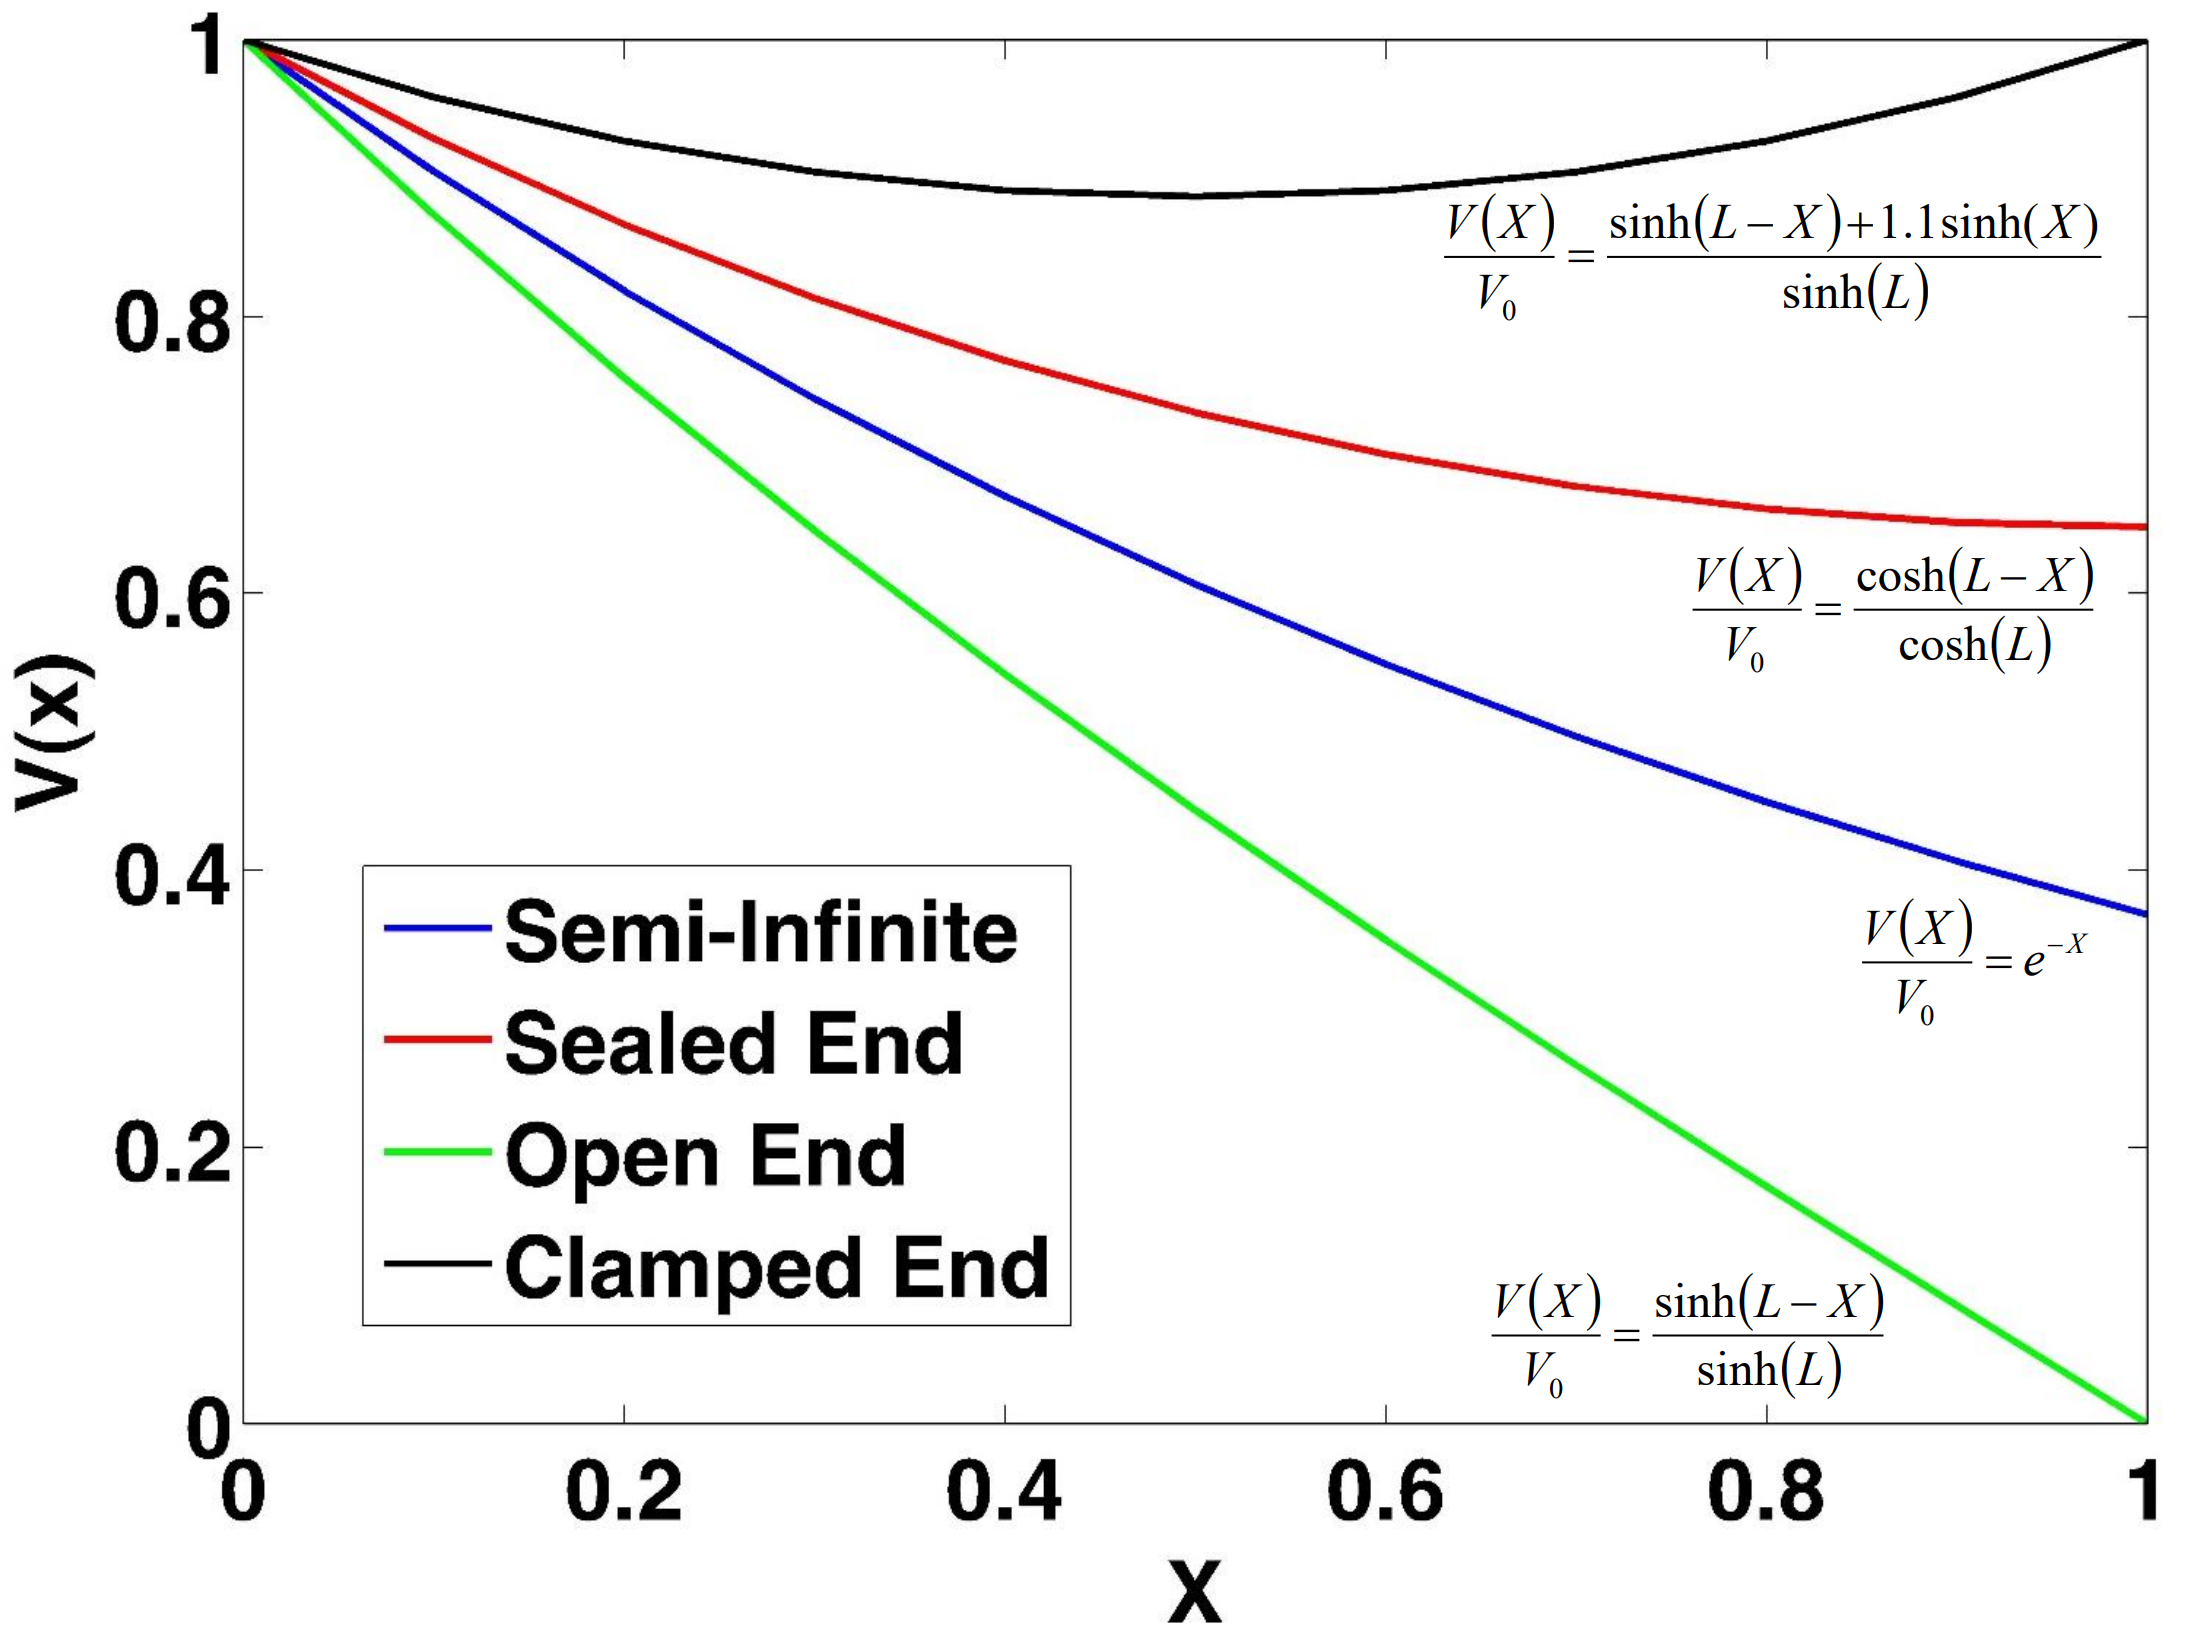
\includegraphics[scale=0.25]{04_6}
    \centering
\end{figure}
Finally, there are also two other cases of finite cable that should be taken into
account:
\begin{itemize}
    \item \textbf{Finite Cable with Leaky End}: the boundary conditions are defined
    by the same expression
    \begin{equation*}
        \pm{\frac{1}{r_{i}}\frac{\partial{V}}{\partial{x}}}\mid{}_{x=0,L}=G_{L}\cdot{V(x,t)}
    \end{equation*}
    with \(G_{L}\) being a conductance which connects the end of the cable to the resting
    potential \(E_{r}\).
    \item \textbf{Finite Cable with Current Injected at Sealed End}: the boundary conditions
    are defined by the same expression
    \begin{equation*}
        \pm{\frac{1}{r_{i}}\frac{\partial{V}}{\partial{x}}}\mid{}_{x=0,L}=I(t)
    \end{equation*}
\end{itemize}
Notice that this is used to model a dendrite stimulated from one extremity to the other
and vice-versa, in order to obtain information on the dendrite properties (collision test).
\subsubsection{Cable Equation Time-Dependent Solutions}
Firstly, let's make an hypothesis: the membrane potential is isopotential, thus it
is constant across the space, in other words \(\frac{\partial{V}}{\partial{X}}=0\).
Said so, the cable equation is simplified as follow:
\begin{equation*}
    \cancel{\frac{\partial^{2}{V}}{\partial{X^{2}}}}-V-\frac{\partial{V}}{\partial{T}}=0
    \Rightarrow
    \frac{\partial^{2}{V}}{\partial{T^{2}}}+V=0
\end{equation*}
If an isopotential neuron is stimulated by a current pulse \(I_{0}\), then:
\begin{equation*}
    V(T)=I_{0}R_{m}(1-e^{-T})
\end{equation*}
where \(R_{m}\) is the membrane resistance of the isopotential segment.\\
Whenever the stimulus is removed, the voltage decays exponentially from
its maximum value \(V(t_{0})=V_{0}\):
\begin{equation*}
    V(T)=V_{0}e^{-T}=V_{0}e^{-\frac{t}{\tau}}
\end{equation*}
In the general case of passive cylinders, thus considering both space and
time constants, the solution of the cable equation \(V(X,T)\) can be expressed as
a sum of an infinite number of exponential decays.

\subsection{The Computational Properties of Dendrites}
When talking about dendrites one may ask whether they are somehow
important from the functional point of view or, on the other hand,
if they play only a key role in forming connections, without any
contribution in computations. With respect to how the brain process
information there are two main viewpoints:
\begin{itemize}
    \item Information processing results primarily from the properties of
    synapses and the connectivity of neurons. The contribution of a single
    neuron is negligible, the emphasis is on the complexity of the overall
    network.
    \item The focus should be on the neuron, playing a fundamental role in the
    computations, thanks to its complex morphology.
\end{itemize}
This second viewpoint is a little old-fashioned nowadays, as it was at the base
of the perceptrons, which aimed at describing the biological neurons and their
computational capabilities in a comprehensive way. The idea was that neurons are
able to operate as devices where analog computations are at a certain point
transformed into a digital output signal.\\
However, today it is mostly believed that linear and non-linear mechanisms
in the dendritic tree are likely to serve as computational building blocks:
combined together they play a key role in the overall computation performed
by a neuron.
\subsubsection{Passive Dendrites}
\paragraph{Passive Filters} They may act as linear filters acting on the input signal: this
kind of filtering tends to attenuate the dendritic signal as a function of the travelled
distance and its frequency. As a consequence, if a signal is too low in power or very
far away it tends to be disregarded.
\paragraph{Non-linear Interactions} Whenever excitatory and inhibitory inputs are
widely separated from one another on different dendritic branches, the input signals
will tend to sum linearly at the soma (a logic OR).\\
If the inputs are adjacent to each other the inhibition can produce a highly non-linear
shunting of the excitatory input (a logic AND-NOT).\\
Moreover, the branch points in the dendritic tree sums up the currents in individual
branches.
\paragraph{Reducing and Amplifying the Mutual Interaction} Generally, excitatory
inputs to the same branch tend to sum sublinearly, whereas inputs on different branches
sum linearly.
\paragraph{Coincidence Detection} The back-propagation of action potentials triggers
a dendritic Ca\({}^{2+}\) spike which depolarizes the whole apical dendrite and drives
a burst of spikes in the axon.
\begin{figure}[H]
    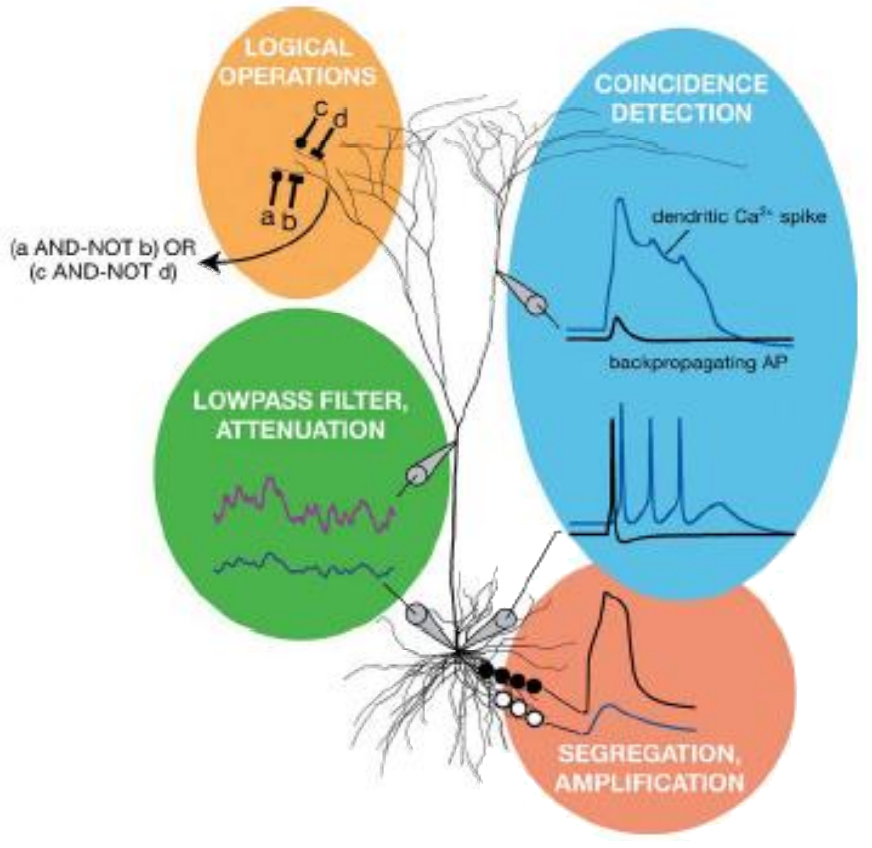
\includegraphics[scale=0.5]{04_7}
    \centering
\end{figure}
\subsubsection{Active Dendrites}
\paragraph{Dynamic Polarization Law} In the nervous system information flows in one
direction, from dendrites to the soma and then to the axon.
\paragraph{Back-propagation Theory} The presence of excitable ionic currents in the
dendrites supports dendritic action potentials that travel in the reverse direction
w.r.t. the main one. Therefore, the neuron is no longer considered to be an
open-loop system, but it presents an internal feedback mechanism.\\
In general, the amount of input is critical in defining the direction of
propagation, while the kind of computation performed is a consequence of
the dendritic tree morphology.